\documentclass[letterpaper]{article}
\usepackage{ms1report}
\usepackage[pdftex]{graphicx}
\usepackage{times}
\usepackage{helvet}
\usepackage{courier}
\usepackage[numbers]{natbib}
\pdfinfo{/Title (The Nature of Breath) /Author (Lauria Clarke)}

\title{The Nature of Breath: A Biomimetic Kinetic Sculpture That Breathes}
\author{Lauria Clarke\\ Parsons School of Design, The New School\\ New York, USA\\ clarl404@newschool.edu\\
\newline
\newline
}
\setcounter{secnumdepth}{0}

\begin{document} 
\maketitle

\begin{abstract}
the nature of breath is...
\end{abstract}

\keywords{Keywords}

%------------------------------
\section{Introduction}

% general introduction


Using the human act of breathing as a lens, this work attempts to lay a foundation for inquiry into the relationship between what is considered to be natural and what is or has been alive. While the focus of this work is on a specifically human form of breath, respiration in broader context is omnipresent in living organisms and is therefore an apt biological process with which to address this question.  

% Respiration is an indicator of life at all scales - from single celled organisms to human beings. Whether involving oxygen in the conventional sense of breath, or operating at the cellular level, the process of energy production is essential to life as we know it. Taking breath, the most natural of human movements, into close consideration, this work examines the relationship between what is natural and what is, or has been, alive.

% With each human breath on this planet we move deeper into the anthropocene.

With the exception of cellular respiration, respiration in breathing organisms is a visibly mechanical process. Humans have created many mechanisms to mimic various aspects of the respiratory system for purposes ranging from medical devices, underwater exploration, to speech synthesis and more. Most of these devices are higly specialized and seek to mimic partifulatr aspects of respiration such as oxygen delivery, or vocal modulation. These works rarely mimic the actual mechanics of the components of the human body responsible for resporation favoring more abstracted and efficient mechanical systems to achieve their goal. Using the freedom afforded by kinetic sculpture, this work attempts to blend a human-biomimetic approach -- highlighting the mehcnical simplicity of the human body -- with a highly technical approach which allows for precise and complex control over the resulting breath.    

This work also asks us to consider the fragility of human breath in light of the COVID-19 pandemic. Seemingly overnight, much of the world became obsessed with breath as the tool of the virus spread. In the two years since, we have become incredibly attuned to the quality and sound of our own breath and what it may say about our mortality. This work seeks to probe these newfound sensitivities, forcing us to question which actions may lead breath to be easy or sharpy painful. 


% Something about being alive. \cite{zimmer}


\subsection{temporal relevance}
% the pandemic...the soundscape of the pandemic...
Teh COVID-19 pandemic has caused a sort of crystalization on many of the aforementioned optics, and has  

During the pandemic many people tried ot mkae ventilators at home. Segue...

\subsection{prior work and relevance}
% talk about the history of breathing apparatus and note that none mimic the human body
Mechanical ventilation has been around for a long time... Since it  seeks to provide "replacement of the respiratory muscles". \cite{ventilatorhistory} This results in apparati that resembly the respiratory system only in the sens that they cause a regutaled chnage in pressure, but have no need for recreating htep rocess by which breaht sounds are actually created. Simialrly, the cield of biomemtic robotics has little use for such inquiry - respiration is not necessary for an electronic humanoid and it is much easier to produce vocal noises in a digital manner. 

Two notable works in the field of kinetic sculpture provide reference, Maywa Denkye's lauching machine and another guy's breath machine thing. These two pieces provoke thought about breath, but still use simple bellow bases mechanisms to produce airflow. %\cite{deynke} \cite{otherguy} 

Since the focus of this piece is the noise of breath 



\section{implementation}

\subsection{system breakdown}

While the avian respiratory system is, in fact, more complex, the human respiratory system is a very complicated biological system. \cite{breathcomplexity} To simplify this system for translation to a constructable mechanical structure, I broke it down into three main sub-systems. Each sub-system exists solely for the purpose of generating breath noises and not for the actual exchnage of oxygen as would normally occur during respiration.  

\subsubsection{Actuation}

Actuation is the system which causes air to move through the respiratory system. In our own bodies this is acieved by the movemne of the diaphgragm. In ventilators this is ofent acieved by a pump or bellows.

\subsubsection{Storage}

Storage describes the way air is stored and contained during the act of breath. This is done by the lungs and is only necessary for the transfer of oxygen to the blood. While the lungs are arguably the most critical part of the respiratory system, they are the most difficult to simulate with accuracy and have relatively little bearing on the sound of breath in this context. 

\subsubsection{Modulation}

Modulation is the way the sound of breath is shaped as it leaves the body. This is acheived by the bronchial tree, trachea, larynx, and mouth. After actuation has been achieved, simulation of this system ist he most relevant and interesting part of this.   

\subsection{making}

So far a few different protptypes ahve been attempted. Focusing on the two main areas of inquiry, there have been auditory prototypes -- exploring the effect os disembodied breath noises -- as well as machnical prototypes -- exploring ways to achieve a physiologically accurate breahting mechanism. 

\subsubsection{auditory prototypes}

bucket experiement

p5 thing

\subsubsection{physical prototypes}

trachea

diaphragm

lever adjustment

\subsubsection{final prototypes}

the final result was a thing that nearly works and combines many of the elements from above

\section{further work}

there's always more to do...

the boris vian reference 


\section{conclusion}

The complexity of the human respiratory system lies not in its gross mechanics, but in the materials and molecular mechanics that allow for the transfer of oxyneg to the blood. The goal of this work was to isolate the mechanical components which form the noise created by breathing.  


talk about the big distinction of artificial and natural

why it's important to think about this in the context of humanity's relationship with the natural world


%\begin{figure}[h]
%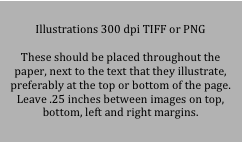
\includegraphics[width=3.31in]{figure.png}
%\caption{This is an example of figure caption. Note that all figures, and tables are to be referenced in the text. \copyright Respect Copyright.}
%\end{figure}
%
%\begin{figure*}
%
\includegraphics[width=\textwidth]{two-column-figure.png}
%\caption{Example of a double-column figure with caption. \copyright Respect Copyright.}
%\end{figure*}


\bibliographystyle{plain}
\bibliography{ms1report}

\section{Bibliography}
%The difference between a reference list and a bibliography is that in your references, you list all the sources you directly referred to in the body of your writing in numerical order, whereas a bibliography includes an alphabetical listing of all those authors and sources that you have consulted while writing your essay. Use the same format as for the references otherwise. Those using Latex will follow the usual cite command format.

\section{Author Biography}
Lauria Clarke is an engineer and artist living in New York. She completed an MS in Computer Engineering at Northeastern University in 2017 and is currently persuing an MFA in Design and Technology at The Parsons School of Design. She specializes in digital hardware design and kinetic sculpture and is always curious to learn more about humanity's relationship with the natural world.

% aspires to be a chocolate fish fisherman for Ben and Jerry's.


\end{document}


% Masahiro Mori's 1970 essay prvided the framework for describing the confusing relationship between artifically created human-like robots and, as Mori calls us, real human beings. \cite{mori} This framework of thought has gained significant traction over the last 50 plus years as developments in technology have made it possiblt to mimic the human body with increasing accuracy. This definition has also been critical in the field of computer science as we consinute ot refine mahcine learning techniques which steadily approach the capacities of the uhman brain. This framework describes the point at which an artificial automaton approaches a point of being eeriely similar to a human being, creating a feeling of discomfort via the uncertainty of whether it is "real".

% For the lats fifty years this framework fo thought has been critical in describing technology's relationship with humanity. 

% Over the last *** years however, the fields of biodesign and bioart have increasingly been asking similar questions not about tchnology and humanity, but technology and nature. In light of the increasing environmental pressures of human imposed climate change, these questions are becoming increasingly urgent. Technology is now being used t oreplicate and mimic natural systems. As Donna Haraway noted in her paper, we must thin kbeyond the human. \cite{haraway} The capacity of our technology has surpassed the instinctually introspective and can now mimic what is natural outside of ourselves. This is a critical development and harkens back to mode indigenous ways of thinking - moving and working with natural systems, rather than in opposition to. 

% If our relationship with technology is extending beyond the human so to must our language. Mori's framework is distinctly human centric. How then do we apply this thinking to non-human natural world? Is Mori's valley merely a snaller depression within a much broader valley encompassing the whole of the natural world? Do humans deserve a place in that broader cintext? To frame this question more broadly, how do we, as human beings, distinguish between what is natural and what is atrificial? How is this distinction shifting as our techological capacity for the artifical increases at great cost to the natural world. 

%While its focus is on a specifically human foram of respiration, respiration in broader context is omnipresent in living organisms, thus providing a jumping off point for larger scope of inquiry into the relationship between what it means to be alive and what it means to be natural. Something about being alive. \cite{zimmer}
